\documentclass[tikz,border=5pt]{standalone}
\begin{document}

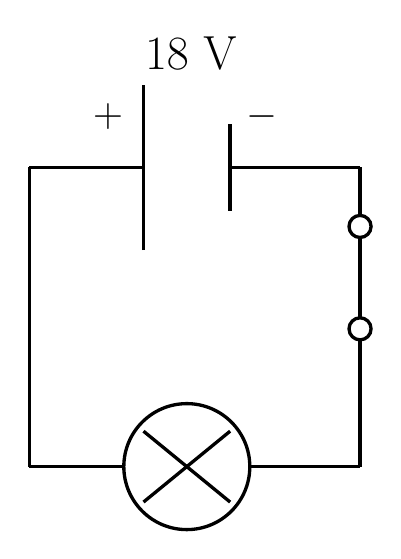
\begin{tikzpicture}[line width=1.2pt]

    % --- Coordonnées utiles ---
    \def\ytop{3.8}
    \def\ybot{0}
    \def\xleft{0}
    \def\xright{4.2}

    % Position de la lampe
    \def\xlamp{2.0}
    \def\rlamp{0.8}

    % Pile
    \def\xbatA{1.45}   % grande plaque
    \def\xbatB{2.55}   % petite plaque

    % --- Fils du circuit ---
    \draw (\xleft,\ybot) -- (\xleft,\ytop);             % côté gauche
    \draw (\xleft,\ytop) -- (\xbatA,\ytop);             % fil haut gauche
    \draw (\xbatB,\ytop) -- (\xright,\ytop);            % fil haut droit

    % côté droit avec deux bornes
    \draw (\xright,\ytop) -- (\xright,3.2);
    \draw (\xright,2.9) -- (\xright,1.9);
    \draw (\xright,1.6) -- (\xright,\ybot);

    % fil bas jusqu'à la lampe
    \draw (\xleft,\ybot) -- (\xlamp-\rlamp,\ybot);
    \draw (\xlamp+\rlamp,\ybot) -- (\xright,\ybot);

    % --- Pile ---
    \draw (\xbatA,\ytop-1.05) -- (\xbatA,\ytop+1.05);   % grande plaque
    \draw (\xbatB,\ytop-0.55) -- (\xbatB,\ytop+0.55);   % petite plaque

    % --- Signes + et - ---
    % Use standard LaTeX sizing commands to avoid unavailable font shapes
    \node[font=\Large] at (1.00,4.45) {$+$};
    \node[font=\Large] at (2.95,4.45) {$-$};

    % --- Texte 18 V ---
    \node[font=\LARGE] at (2.05,5.25) {18 V};

    % --- Bornes à droite ---
    \draw (\xright,3.05) circle (0.14);
    \draw (\xright,1.75) circle (0.14);

    % --- Lampe ---
    \draw (\xlamp,\ybot) circle (\rlamp);
    \draw (\xlamp-0.55,\ybot+0.45) -- (\xlamp+0.55,\ybot-0.45);
    \draw (\xlamp-0.55,\ybot-0.45) -- (\xlamp+0.55,\ybot+0.45);

\end{tikzpicture}

\end{document}